\begin{ledgroupsized}[r]{120mm}
\footnotesize 
\pstart 
\noindent\textbf{\"{U}berlieferung:}
\pend
\end{ledgroupsized}
\begin{ledgroupsized}[r]{114mm}
\footnotesize 
\pstart \parindent -6mm
\makebox[6mm][l]{\textit{L}}%
Aufzeichnung:
 LH XXXVII 4 Bl. 49-50.
1 Bog. 2\textsuperscript{o}.
Etwa 1 S. auf Bl. 50~v\textsuperscript{o}.
Die letzten 4 Z. % von Bl. 50~v\textsuperscript{o}
überliefern N.~88.
% 037,04_049 = Mittel, einen warmen Wind ...
Bl. 50~r\textsuperscript{o} ist leer.
Bl. 49 überliefert N.~42. Ein Wasserzeichen
% 037,04_050 = Cc2 972 = Demonstratio de trabis aequilibrio
 auf Bl.~49.\\%
Cc 2, Nr. 973  (tlw.)
\pend
\end{ledgroupsized}
%
\vspace*{5mm}
\begin{ledgroup}
\footnotesize 
\pstart
\noindent\footnotesize{\textbf{Datierungsgr\"{u}nde:}
Das vorliegende Stück N.~43 ist auf demselben Bogen überliefert wie das Stück N.~42. % 037,04_050 = Cc2 972 = Demonstratio de trabis aequilibrio
Dieses letztere ist editorisch auf September 1672 bis März 1673 datiert (siehe die Begründung dort).
Die für N.~42 vorgeschlagene Datierung wird demgemäß auch für N.~43 übernommen.}
\pend
\end{ledgroup}
%
\count\Afootins=1200
\count\Bfootins=1200
\count\Cfootins=1200
\vspace*{8mm}%
\pstart%
\noindent%
\normalsize%
% [50~v\textsuperscript{o}]
[50~v\textsuperscript{o}] 
\edtext{Omne flexile}{\lemma{Omne}\Bfootnote{\textit{(1)} filum hab \textit{(2)} flexile \textit{L}}} \edtext{naturale}{\lemma{}\Bfootnote{naturale \textit{erg. L}}} Elasticum\protect\index{Sachverzeichnis}{elasticum} est. Experimento id probatur, sumatur filum quodcunque ex eo pendat pondus, quod circumagatur, hoc facto filum repellet pondus et aperiet sese et multis spiris aget in contrariam partem, ubi rursus comprimet ultra modum, et rursus repelletur.\pend 
\pstart Magnum est discrimen inter Naturalia et artificialia, flexilia, cohaerentia, liquida, perspicua, \edtext{figurata. Naturalia qualia sunt}{\lemma{figurata.}\Bfootnote{\textit{(1)}\ Perspicua naturalia, sunt per mi \textit{(2)}\ Naturalia qualia sunt \textit{L}}} \edtext{plerumque}{\lemma{}\Bfootnote{plerumque \textit{erg. L}}} per minima sunt, artificialia, per partes, relictis intervallis heterogeneis. Omnia perspicua naturalia refringunt, artificialia non refringunt. Flexilia naturalia Elastica sunt. Liquida naturalia (artificiale est pulvis) habent aliquam cohaesionem. Omnia cohaerentia naturalia tendibilia \edlabel{flexile1}sunt.
\pend
\pstart%
\edtext{Guttae\edlabel{flexile2}}{{\xxref{flexile1}{flexile2}}\lemma{sunt.}\Bfootnote{\textit{(1)}\ Sphaerica vera seu \textit{(2)}\ Guttae \textit{L}}} in quas liquida formantur indicium sunt cohaesionis reliquae in ipsis.
\edtext{Galilaeus\protect\index{Namensregister}{\textso{Galilei} (Galilaeus, Galileus), Galileo 1564-1642} in dial. mech. prim. ni fallor refert \edtext{ad circumstantem aerem}{\lemma{ad}\Bfootnote{\textit{(1)}\ aquam \textit{(2)}\ circumstantem aerem \textit{L}}} nescio quam aquae et aeris inimicitiam comminiscens.}{\lemma{Galilaeus [...] comminiscens}\Cfootnote{\cite{00050}\textsc{G. Galilei}, \textit{Discorsi}, Leiden 1638, S. 71f. (\cite{00048}\textit{GO} VIII, S. 115f.).}}
Sed observatum est illas guttulas rotundas manere etiam aere exhausto.
\pend
\pstart
Cur \edtext{guttae liquoris alicujus in Tabula}{\lemma{guttae}\Bfootnote{\textit{(1)}\ in \textit{(a)} planis \textit{(b)} superficie \textit{(2)} liquorem \textit{(3)} liquoris alicujus in Tabula \textit{L}}}
 horizonti parallela, non humida, sed sicca, aut humore aliquo sed humoris stillantis diffusioni obsistente imbuta, rotundentur.
\pend 
\pstart Manifestum est omnes aquae guttas dum cadunt pondere proprio reddi nonnihil oblongas ut \textit{ab} in \edtext{imo}{\lemma{in}\Bfootnote{\textit{(1)}\ basi \textit{(2)}\ imo \textit{L}}} tamen \textit{b} non plana, instar cylindri, sed curva instar ovalis aut Ellipsis quae vero speciatim figura sit, id nihil pertinet ad rem nostram. Attingit ergo planum \textit{c} puncto \textit{b} et eodem tempore pondus superioris, incumbens inferiori conatur massam \textit{ab} procudere in planum quantum \edtext{potest latum}{\lemma{potest}\Bfootnote{\textit{(1)}\ magnum \textit{(2)}\ latum \textit{L}}} sed tenue. \edtext{At huic}{\lemma{tenue.}\Bfootnote{\textit{(1)}\ Sed \textit{(2)}\ At huic \textit{L}}} diffusioni obsistit ipse fundus \textit{c} aliquantulum tamen obtundi, complanarique ipsum \textit{b} necesse est, velut ovo Columbi\protect\index{Namensregister}{\textso{Kolumbus}, Christoph (1451-1506)} marmori laevigato illiso. At reliquum super incumbens cum ultra progredi non possit recta, ibit in latus. Imo jam ab initio statim, quantum enim imum procuditur, tantum summum diffunditur. Quodsi tam exigua ponatur pressio aut tanta fundi resistentia, ut diffusio in \textit{b} per \textit{c} haberi possit pro nulla \edtext{seu ut contactus sit in puncto \textit{b}}{\lemma{}\Bfootnote{seu [...] puncto \textit{b} \textit{erg. L}}} rationis est guttam formari \edtext{in globulum \textit{bef.} Primum enim}{\lemma{}\Bfootnote{in\ \textbar\ globulum \textit{erg.}\ \textbar\ \textit{bef.}\ \textit{(1)}\ Contactus est ut dixi, in puncto. Ergo figura\ \textit{(2)}\ Primum enim\ \textit{L}}} fundus aquam se diffusuram cohibet interea omnia incumbentia superurgent, sed \edtext{obstat descendere}{\lemma{obstat}\Bfootnote{\textit{(1)}\ in fundum \textit{(2)}\ descendere \textit{L}}} conantibus ipsa partium connexio. \edtext{Nota etsi gravitas in specie major connexione. Considerandum tamen an non mutata figura}{\lemma{connexio.}\Bfootnote{\textit{(1)}\ Quae si aequalis gravitati\protect\index{Sachverzeichnis}{gravitas|textit}, fiet mutuo nulla, sed corpus retinebit figuram quam habebat, quodsi major \textit{(2)}\ Nota [...] figura, \textit{L}}}, plus lucretur gravitas\protect\index{Sachverzeichnis}{gravitas}, quam perdit connexio, id est an plures descendant quam separentur; figura conciliatrix ubi plurimum descendit, minima separatione; aut aequilibratur tandem multitudo partium gradui conatuum. Ea denuo figura optima est. Et hanc considerationem nulli in \edtext{mentem venisse memini}{\lemma{mentem}\Bfootnote{\textit{(1)}\ venissem \textit{(2)}\ venisse memini. \textit {L}}}. Sed haec in calculum appendenda sunt per Geometriam indivisibilium sine qua nihil solidi ratiocinari possumus de motu. Ecce hic novum genus compensationis scilicet multitudinis partium per gradum conatus\protect\index{Sachverzeichnis}{conatus} \setline{16}simplicem, seu absolutum, ut alias magnitudinis ad celeritatem.
\pend
%\begin{center}
%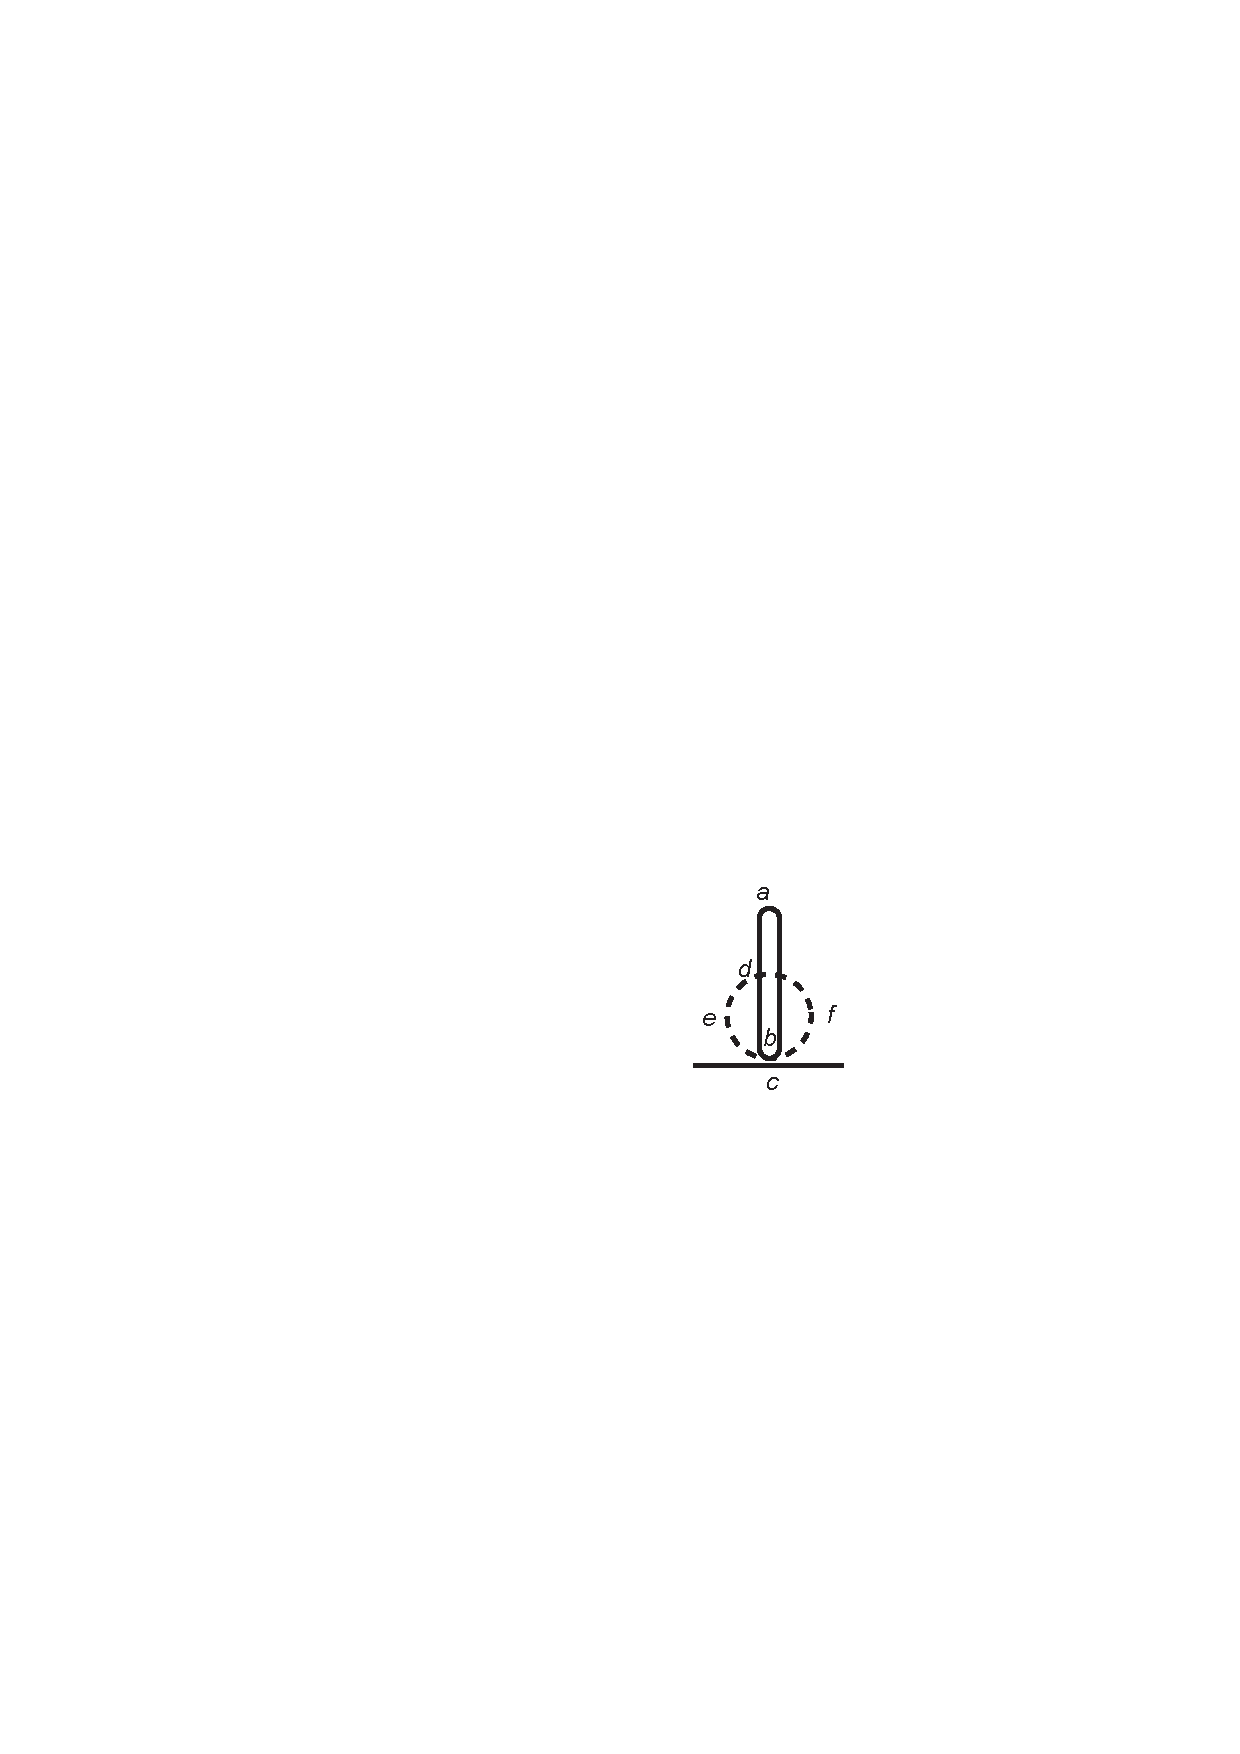
\includegraphics[width=0.18\textwidth]{images/LH03704_50r-d1.pdf}
%\lbrack\textit{Fig. 1}\rbrack
%\hspace{10mm}
%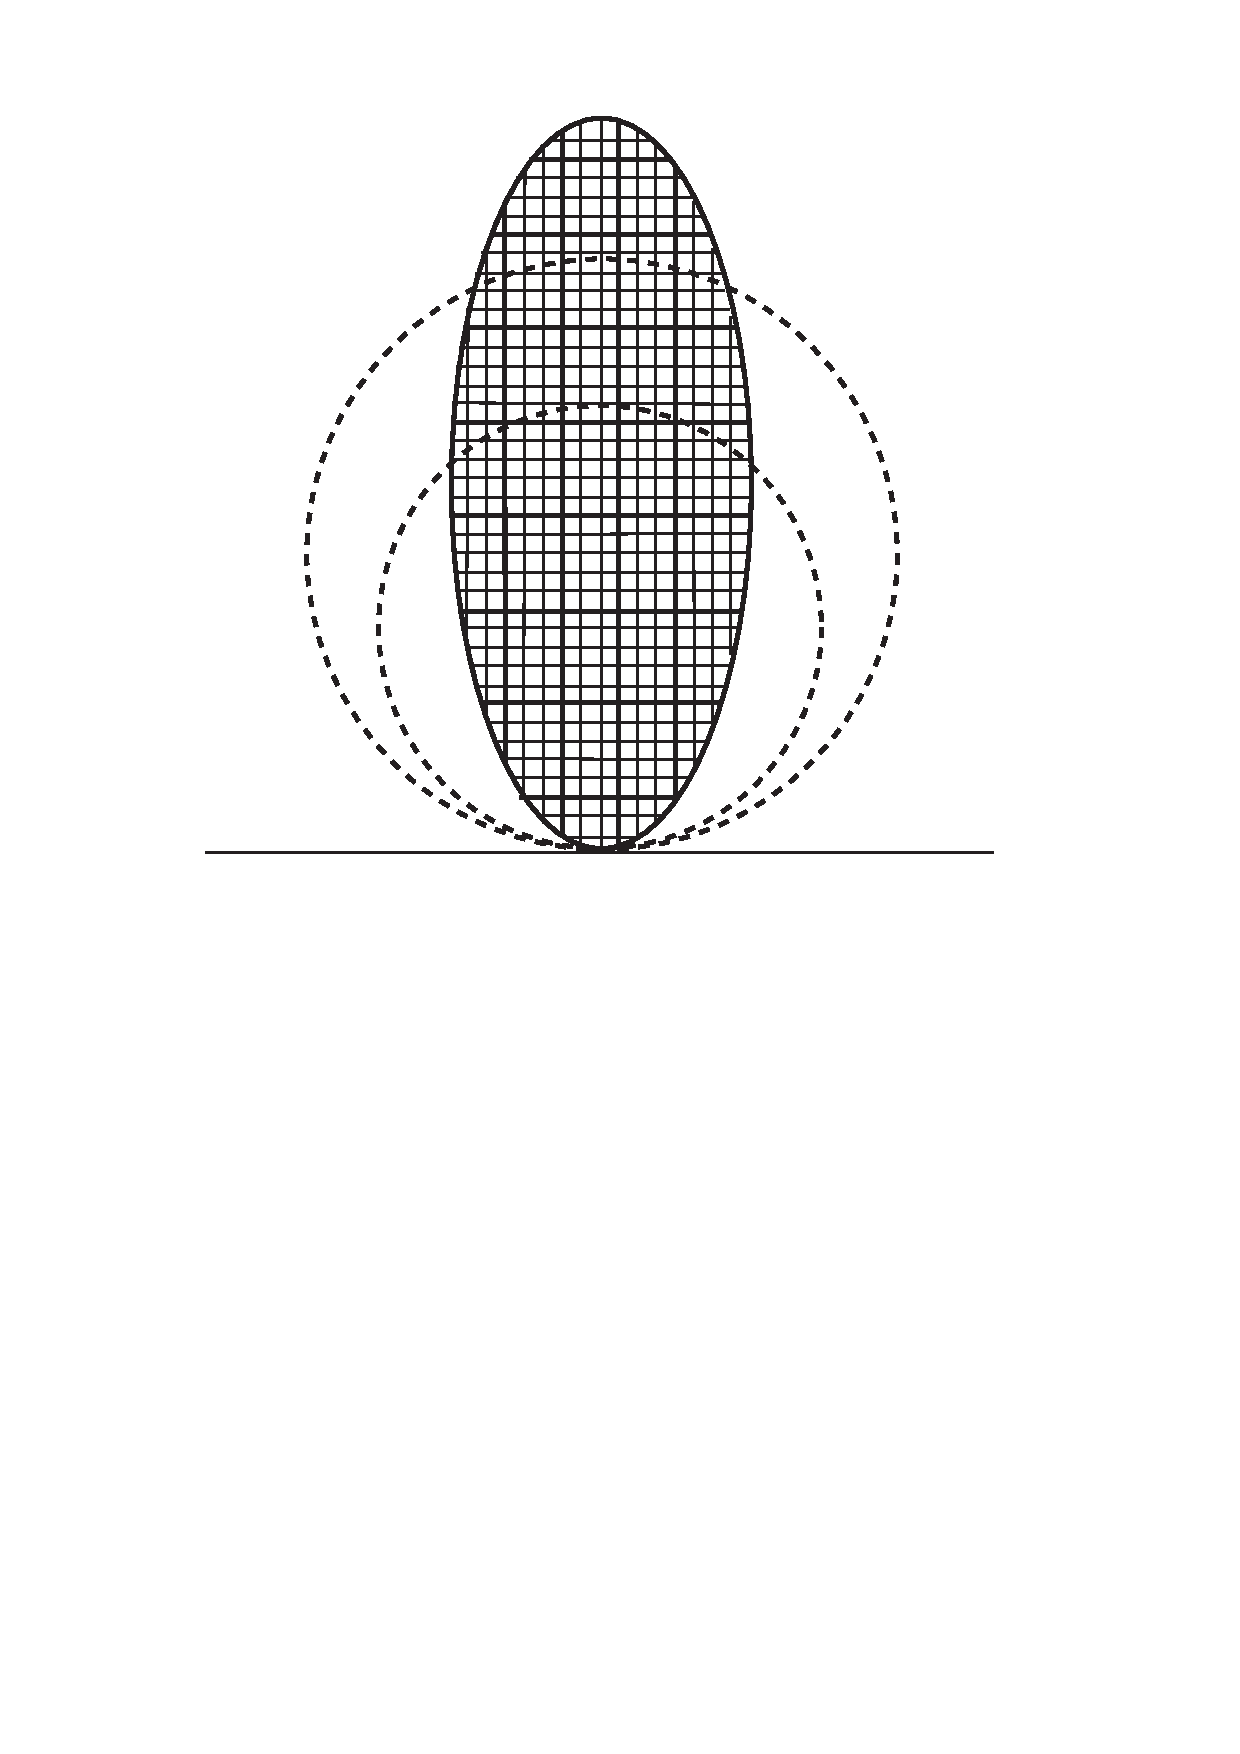
\includegraphics[width=0.38\textwidth]{images/LH03704_50r-d2.pdf}\\
%\rule[0pt]{0mm}{0pt}[\textit{Fig. 1}]\hspace{40mm}[\textit{Fig. 2}]
%\end{center}
\vspace*{3.0em}
\pstart
\noindent
\begin{minipage}[t]{0.5\textwidth}
\hspace*{20mm}
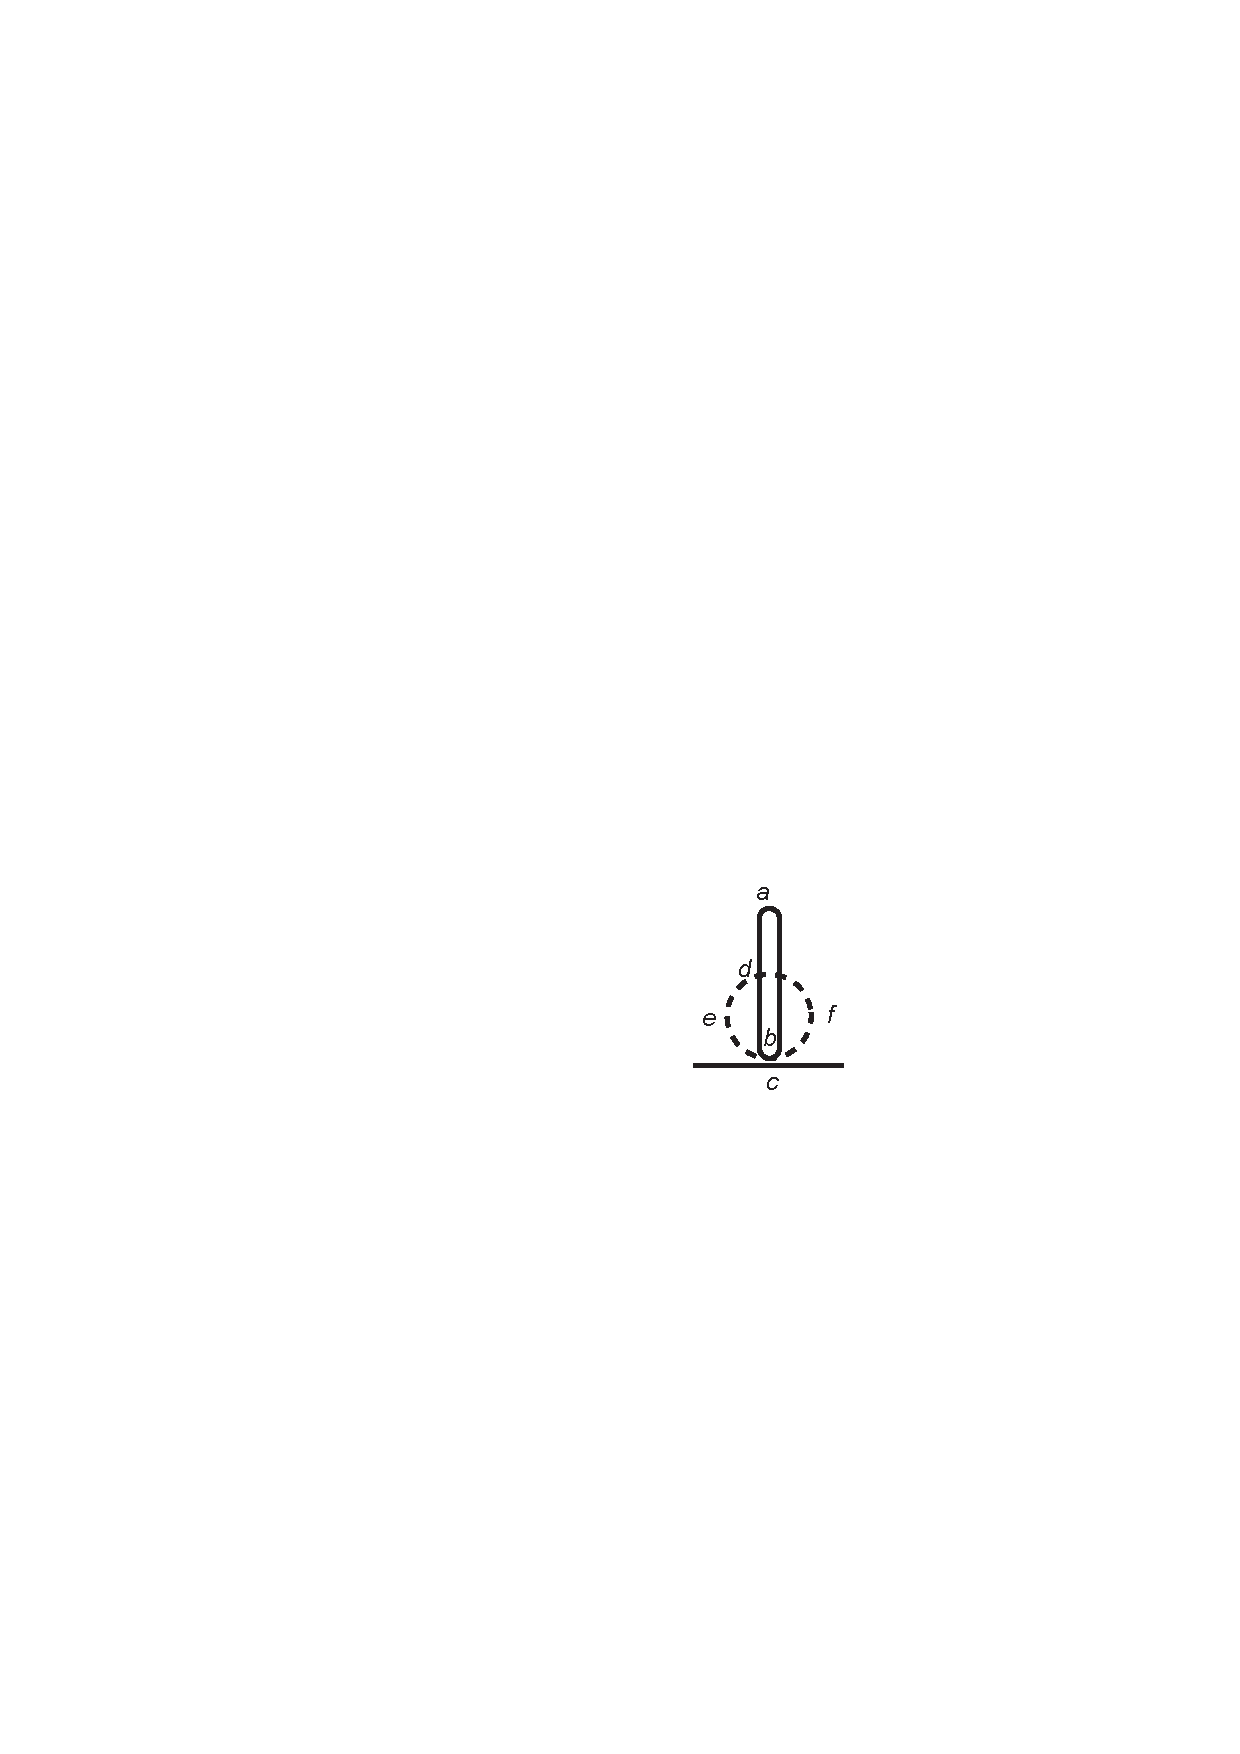
\includegraphics[trim = 0mm 2.9mm 0mm 0mm, clip, width=0.4\textwidth]{images/LH03704_50r-d1.pdf}
\end{minipage}
\hspace{5mm}
\begin{minipage}[t]{0.5\textwidth}
%\hspace*{-5mm}
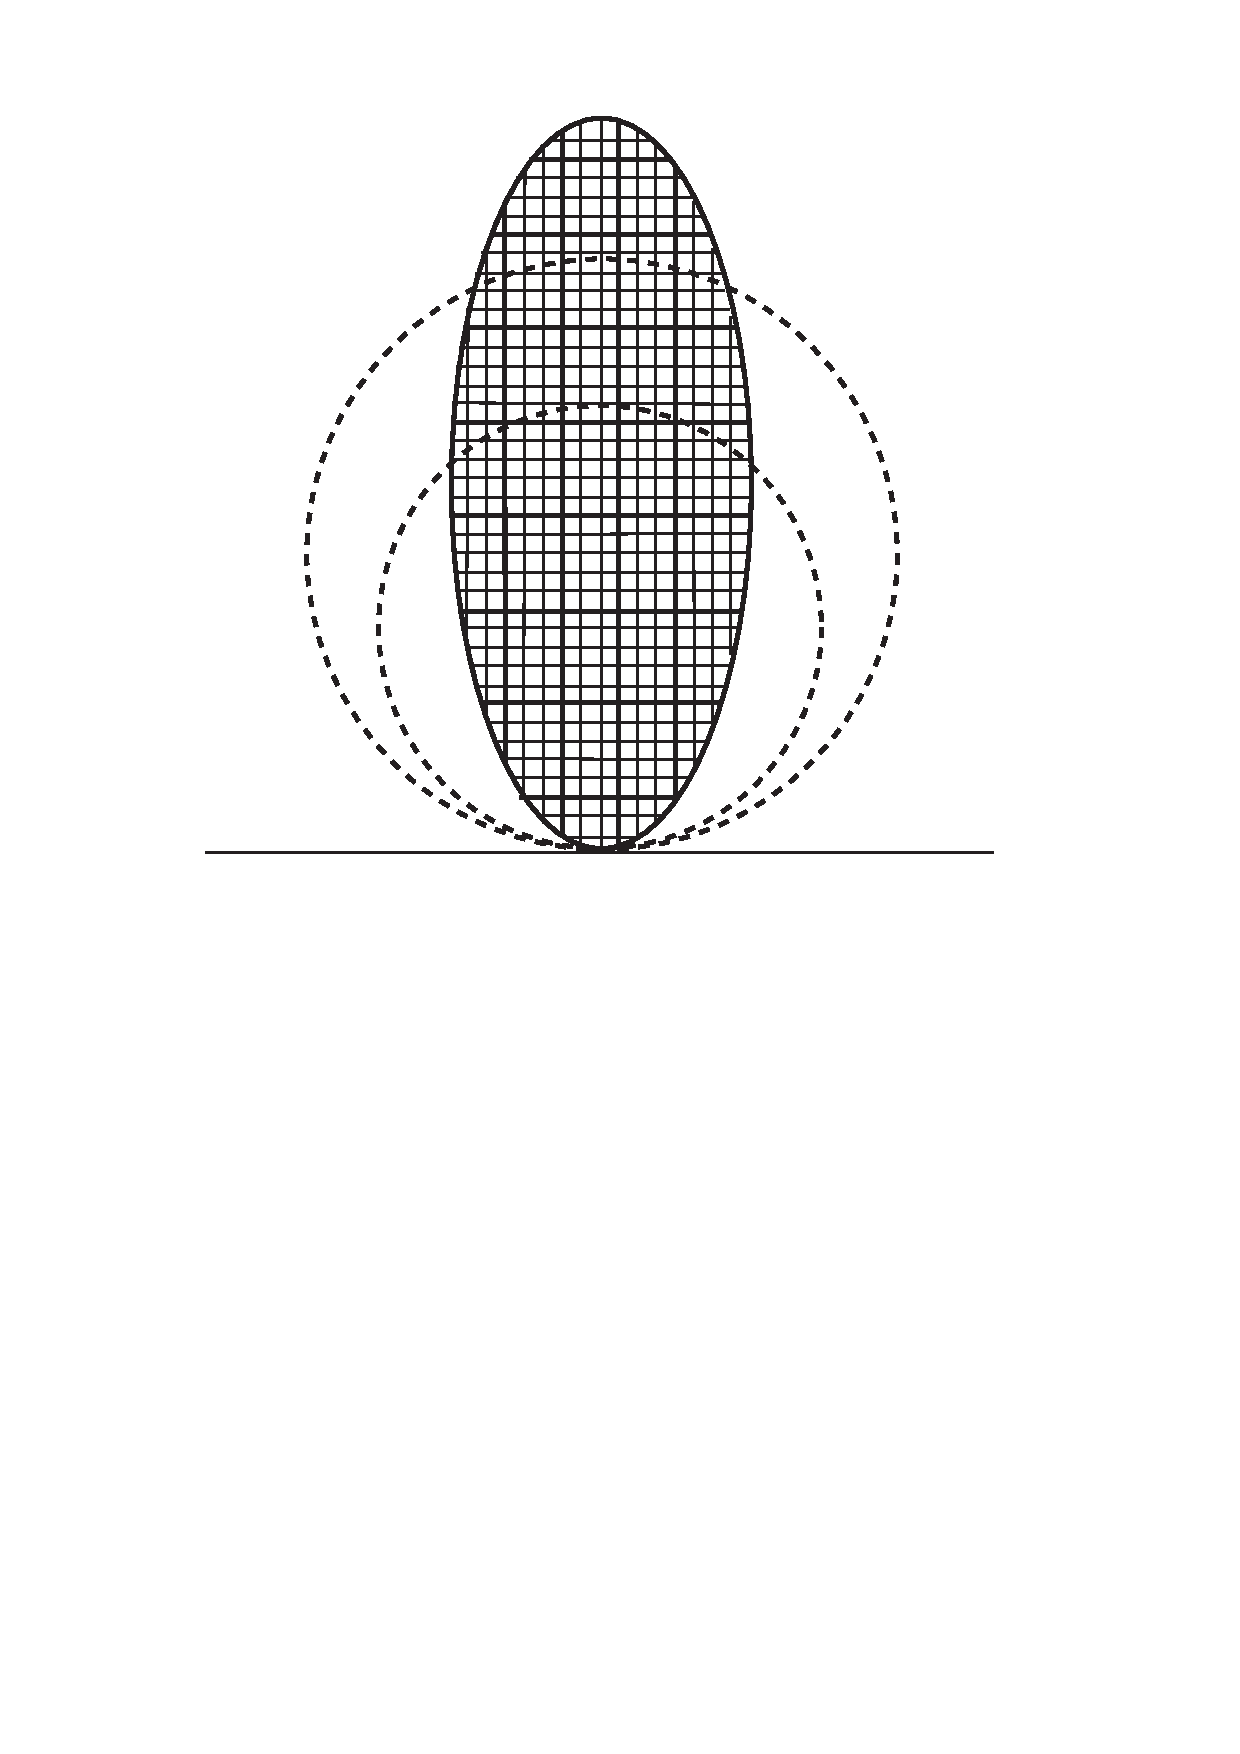
\includegraphics[width=0.5\textwidth]{images/LH03704_50r-d2.pdf}\\
\end{minipage}
%\vspace*{1mm}
\hspace*{28mm} [\textit{Fig. 1}]\hspace*{44mm} [\textit{Fig. 2}]
\pend
\count\Afootins=1500
\count\Bfootins=1500
\count\Cfootins=1500